% Ehemals Test(s).pdf -- ergaenzt um die Pruefung der Version 2.0.0
% Teil A: Testfaelle 1 bis 6 (Version 1.x, 2021, DOS-Box, mit Screenshots)
% Teil B: Modellpruefung 2.0.0 (Dokumentation/Modelltest/modelltest.py)
% Teil C: noch auszufuehrende DOS-Box-Tests fuer 2.0.0

% Hilfsmakros fuer die Tabellen (nur in dieser Datei)
\newcommand{\hexdez}[2]{$#1_{\text{hex}}$ ($#2_{\text{dez}}$)}
\newcommand{\hexs}[1]{$#1_{\text{hex}}$}
\newcommand{\sbrow}[4]{#1 & \hexdez{#2}{#3} & \hexs{#4} & \iconok \\ \hline}
\newcommand{\srrow}[6]{#1 & \hexdez{#2}{#3} & \hexdez{#4}{#5} & \cellcolor{blk#6} #6 \\ \hline}
\newcommand{\sarow}[5]{#1 & \hexdez{#2}{#3} & \hexs{#4} & \hexs{#5} \\ \hline}
\definecolor{blk1}{RGB}{189,215,238}
\definecolor{blk2}{RGB}{255,217,102}
\definecolor{blk3}{RGB}{244,176,132}
\definecolor{blk4}{RGB}{169,208,142}

\section{AES-Tests}\label{sec:tests}
\textit{Abschlussprojekt Modul \glqq Assemblerprogrammierung\grqq{} von Konstantin Blechschmidt \& Tim M.\ Kretzschmar}

\subsection{Überblick und Stand der Prüfung}\label{sec:tests-stand}
Die Tests gliedern sich in drei Teile:
\begin{description}[leftmargin=!,labelwidth=2.2cm,noitemsep]
    \item[Teil A] Die Testfälle 1 bis 6 sind die Tests der \emph{Version~1.x} aus dem Jahr 2021. Sie wurden in der DOS-Box durchgeführt, die Screenshots sind die Belege. Sie bleiben als Dokumentation erhalten, wurden für Version~\versionProjekt\ aber \textbf{nicht wiederholt}.
    \item[Teil B] Die Modellprüfung der Version~\versionProjekt\ (Abschnitt~\ref{sec:tests-modell}): Die Rechenroutinen sind in Python nachgebaut und gegen unabhängige Referenzen geprüft.
    \item[Teil C] Die Tests, die in der DOS-Box für Version~\versionProjekt\ noch nachzuholen sind (Abschnitt~\ref{sec:tests-dosbox}), mit den erwarteten Werten aus Teil~B.
\end{description}

\begin{table}[!htbp]
    \centering
    \small
    \renewcommand{\arraystretch}{1.1}
    \caption{Übersicht der Testfälle aus Version 1.x und ihr Stand in Version \versionProjekt}\label{tab:tests-uebersicht}
    \begin{tabular}{@{}p{5.2cm}cp{6.0cm}@{}}
        \toprule
        \textbf{Testfall (Version 1.x)} & \textbf{Ergebnis 1.x} & \textbf{Stand in \versionProjekt} \\
        \midrule
        1 -- Bildschirmwechsel per Mausklick & \iconok & Code unverändert; DOS-Box-Wiederholung offen \\
        2 -- SBOX-Substitution bei Ver- und Entschlüsseln & \iconok & inverse S-Box geändert (Index \hexs{70}); Modell M1, DOS-Box offen \\
        3 -- ShiftRow \& Inverse & \iconok & \asm{ShiftRow} geändert (vierter Block); Modell M2, DOS-Box offen \\
        4 -- ShiftColumn & \iconok & \asm{MalZweiPROC} geändert; Modell M4, M6, M7 \\
        5 -- ShiftColumn Invers & \iconfehler & \asm{ShiftColumn_1} neu geschrieben; Modell M5--M7 \\
        6 -- SchluesselAnwenden (PROC) & \iconok & unverändert; Schlüsselexpansion neu in M3 \\
        \bottomrule
    \end{tabular}
\end{table}

Die Symbole \iconok{} und \iconfehler{} in dieser Tabelle und in den Testfällen geben das Ergebnis der \emph{damaligen} Tests an. Sie sagen nichts über Version~\versionProjekt\ aus.

%------------------------------------------------------------------------------
\subsection{Testfall 1 -- Bildschirmwechsel per Mausklick}\label{sec:tf1}
\begin{figure}[H]
    \noindent\textbf{Hauptbildschirm:}\par\vspace{2mm}
    \centering
    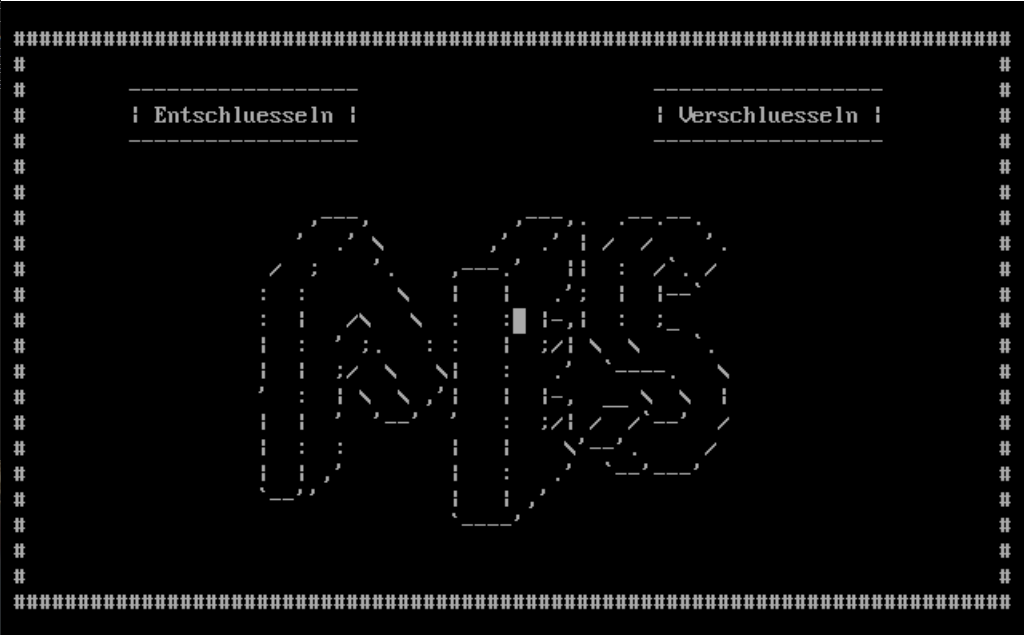
\includegraphics[width=0.72\textwidth]{images/tf1_hauptbildschirm.png}
    \caption{Hauptbildschirm -- der Cursor befindet sich in der Bildschirm-Mitte}
    \label{fig:tf1-haupt}
\end{figure}

\begin{figure}[H]
    \noindent\textbf{Maus über der Verschlüsselung:}\par\vspace{2mm}
    \centering
    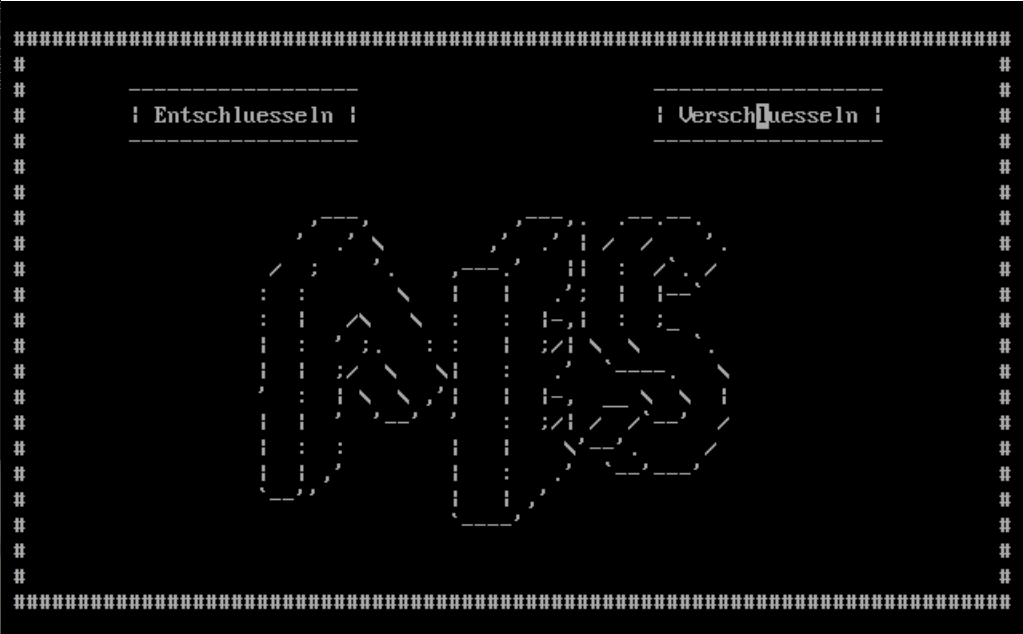
\includegraphics[width=0.72\textwidth]{images/tf1_maus_ueber_ver.png}
    \caption{Cursor über der Schaltfläche \glqq Verschluesseln\grqq}
    \label{fig:tf1-maus}
\end{figure}

\begin{figure}[H]
    \noindent\textbf{Nach dem Klick:}\par\vspace{2mm}
    \centering
    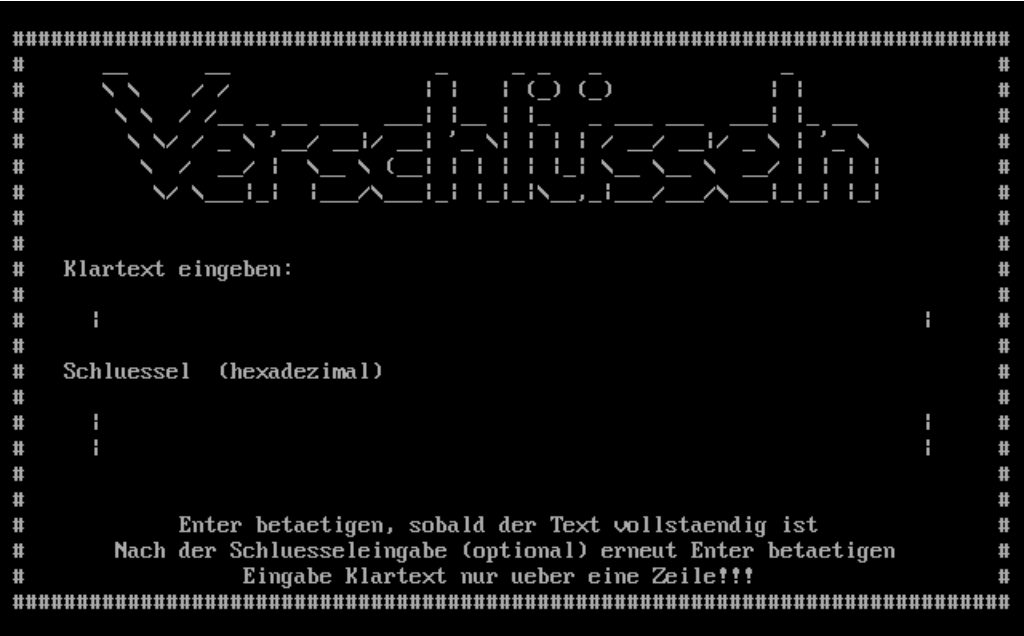
\includegraphics[width=0.72\textwidth]{images/tf1_nach_klick.png}
    \caption{Bildschirm nach dem Klick auf \glqq Verschluesseln\grqq}
    \label{fig:tf1-klick}
\end{figure}

%------------------------------------------------------------------------------
\Needspace{14\baselineskip}
\subsection{Testfall 2 -- SBOX-Substitution bei Ver- und Entschlüsseln}\label{sec:tf2}
\begin{figure}[H]
    \noindent\textbf{Eingabe Verschlüsselung}\par\vspace{2mm}
    \centering
    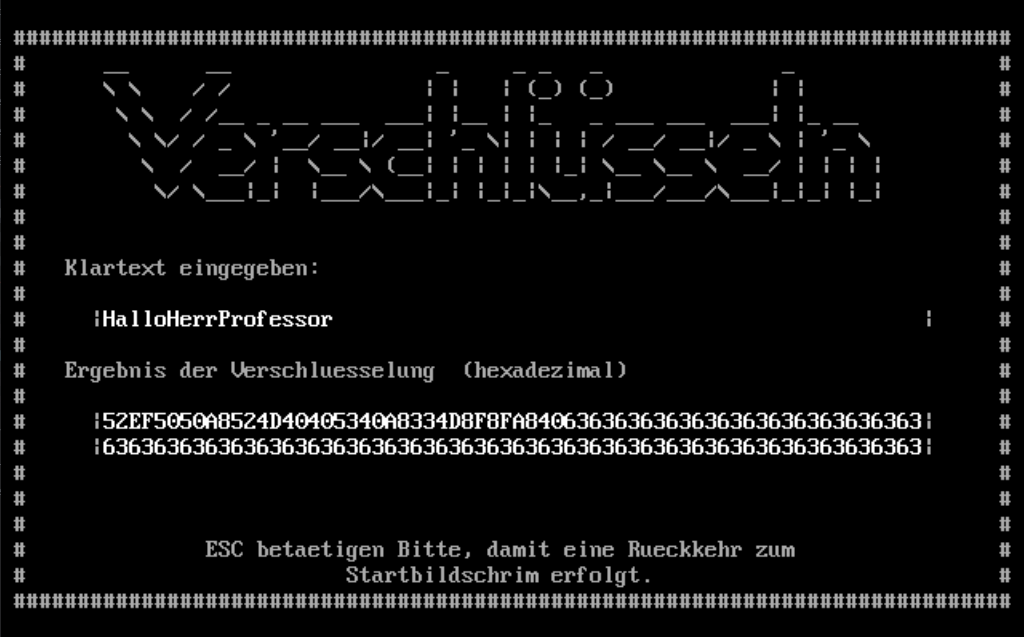
\includegraphics[width=0.72\textwidth]{images/tf2_ver_eingabe.png}
    \caption{Testfall 2: Eingabe \glqq HalloHerrProfessor\grqq{} und Ergebnis der Verschlüsselung}
    \label{fig:tf2-ver}
\end{figure}

\begin{table}[H]
    \noindent\textbf{Beweis:}\par\vspace{2mm}
    \centering
    \small
    \renewcommand{\arraystretch}{1.05}
    \caption{Testfall 2: SBOX-Substitution}\label{tab:tf2}
    \begin{tabular}{|l|l|l|c|}
        \hline
        \textbf{Buchstabe} & \textbf{HexWert (ASCII)} & \textbf{Substitutionswert} & \\ \hline
        \sbrow{H}{48}{72}{52}
        \sbrow{a}{61}{97}{EF}
        \sbrow{l}{6C}{108}{50}
        \sbrow{l}{6C}{108}{50}
        \sbrow{o}{6F}{111}{A8}
        \sbrow{H}{48}{72}{52}
        \sbrow{e}{65}{101}{4D}
        \sbrow{r}{72}{114}{40}
        \sbrow{r}{72}{114}{40}
        \sbrow{P}{50}{80}{53}
        \sbrow{r}{72}{114}{40}
        \sbrow{o}{6F}{111}{A8}
        \sbrow{f}{66}{102}{33}
        \sbrow{e}{65}{101}{4D}
        \sbrow{s}{73}{115}{8F}
        \sbrow{s}{73}{115}{8F}
        \sbrow{o}{6F}{111}{A8}
        \sbrow{r}{72}{114}{40}
        \glqq 0\grqq{} (Nicht die ASCII 0) & \hexs{00} & \hexs{63} & \iconok \\ \hline
    \end{tabular}
\end{table}

Die große Menge an \glqq 63\grqq{} nach der Nachricht erscheinen durch den Hintergrund, dass der \asm{TastaturBuffer} (das Array zum Zwischenspeichern) mit 0 initialisiert ist und somit alle nicht überschriebenen Werte eine 0 innehaben.

\begin{figure}[H]
    \noindent\textbf{Gegeneingabe Entschlüsseln}\par\vspace{2mm}
    \centering
    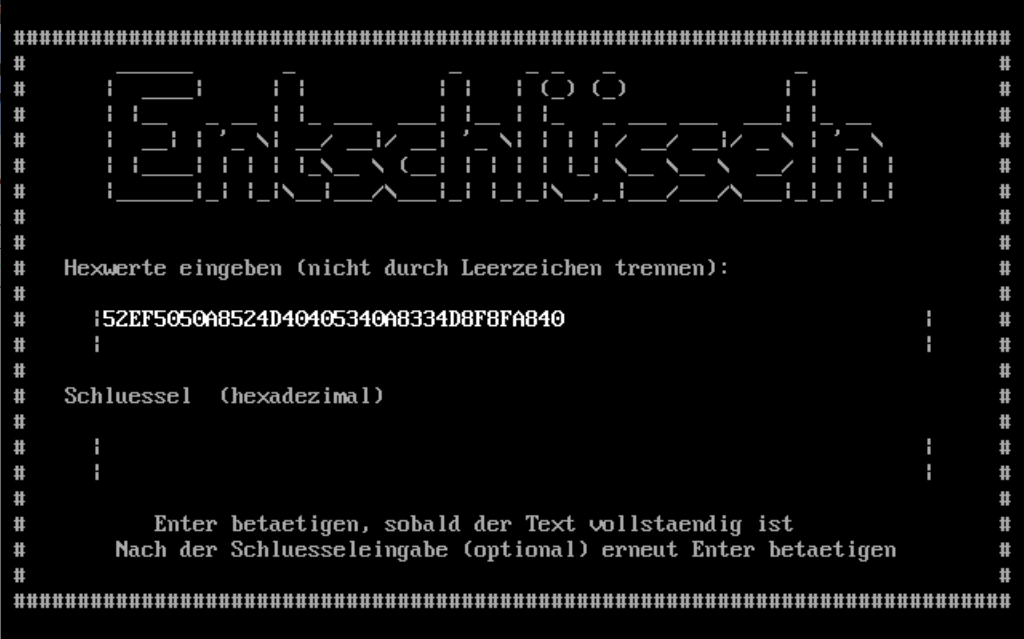
\includegraphics[width=0.72\textwidth]{images/tf2_ent_eingabe.png}
    \caption{Testfall 2: Eingabe des Chiffretextes zum Entschlüsseln}
    \label{fig:tf2-ent-ein}
\end{figure}

\begin{figure}[H]
    \centering
    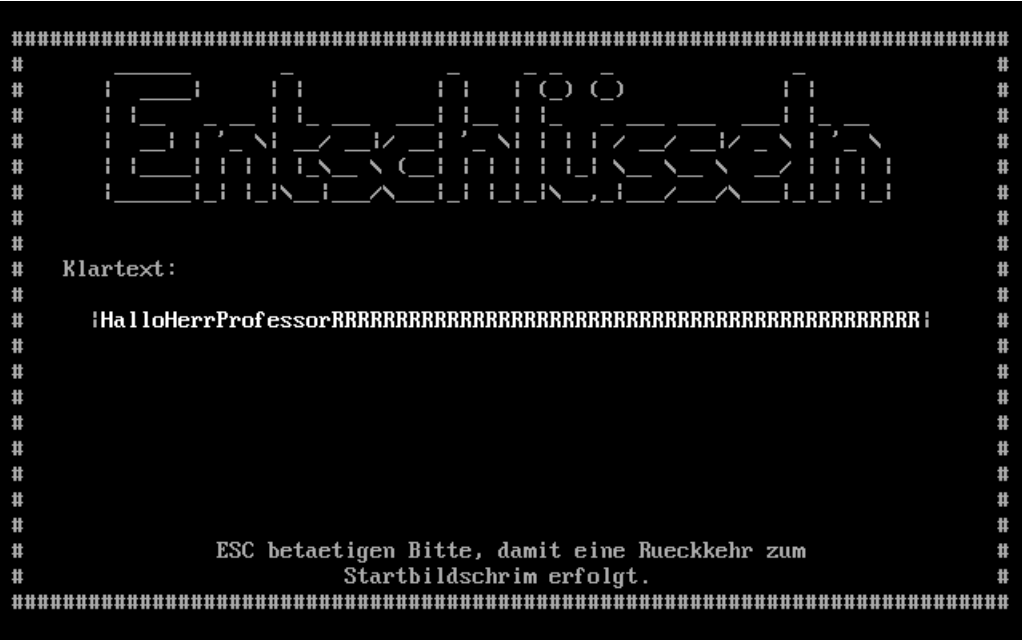
\includegraphics[width=0.72\textwidth]{images/tf2_ent_ergebnis.png}
    \caption{Testfall 2: Ergebnis der Entschlüsselung}
    \label{fig:tf2-ent-erg}
\end{figure}

Die ganzen \glqq R\grqq{} entstehen wieder durch die fehlende Eingabe (0 bei der invertierten SBox ist $52_{\text{hex}}$ und dies entspricht dem großen R).

%------------------------------------------------------------------------------
\Needspace{14\baselineskip}
\subsection{Testfall 3 -- ShiftRow \& Inverse}\label{sec:tf3}
\textbf{Stand 2.0.0:} Der Test war erfolgreich, deckte aber einen Fehler nicht auf: Der Text hat nur 18 Zeichen, der vierte Block (\asm{Pos 48}--\asm{63}) enthält nur Nullbytes, und deren Verschiebung ist unsichtbar. Tatsächlich wurde der vierte Block in 1.x nie verschoben (Abschnitt~\ref{sec:vers-shiftrow}). Seit 2.0.0 ist das behoben; ein Test mit 64 Zeichen steht in Teil~C aus.

\begin{figure}[H]
    \noindent\textbf{Eingabe Verschlüsselung}\par\vspace{2mm}
    \centering
    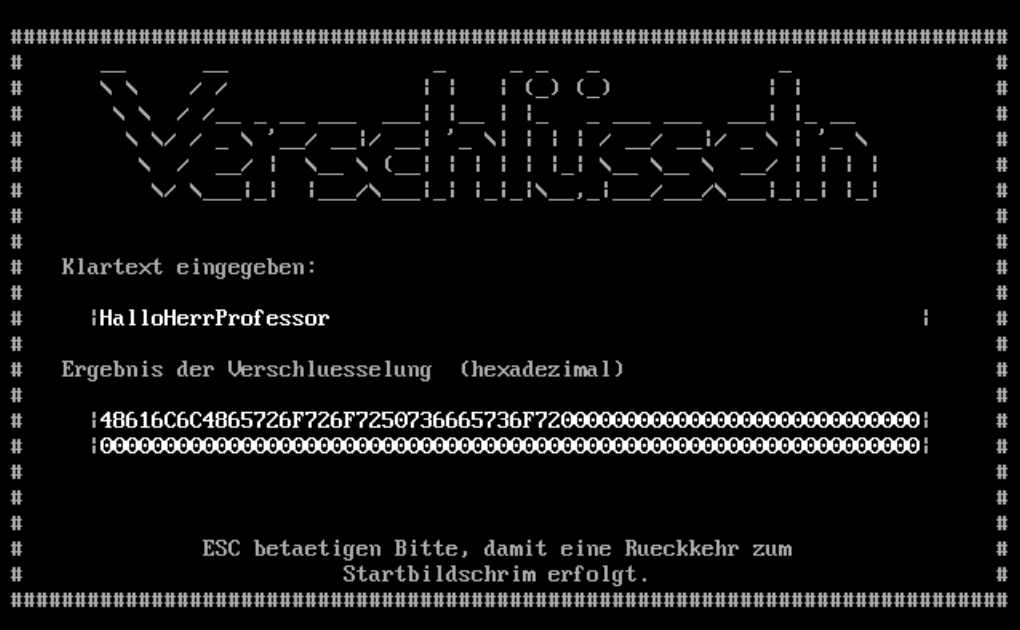
\includegraphics[width=0.72\textwidth]{images/tf3_ver_eingabe.png}
    \caption{Testfall 3: Eingabe \glqq HalloHerrProfessor\grqq{} und Ergebnis}
    \label{fig:tf3-ver}
\end{figure}

\begin{table}[H]
    \noindent\textbf{Beweis:}\par\vspace{2mm}
    \centering
    \small
    \renewcommand{\arraystretch}{1.05}
    \caption{Testfall 3: ShiftRow}\label{tab:tf3}
    \begin{tabular}{|l|l|l|c|}
        \hline
        \textbf{Buchstabe} & \textbf{HexWert (ASCII)} & \textbf{Verschoben} & \textbf{Blöcke} \\ \hline
        \srrow{H}{48}{72}{48}{72}{1}
        \srrow{a}{61}{97}{61}{97}{1}
        \srrow{l}{6C}{108}{6C}{108}{1}
        \srrow{l}{6C}{108}{6C}{108}{1}
        \srrow{o}{6F}{111}{48}{72}{2}
        \srrow{H}{48}{72}{65}{101}{2}
        \srrow{e}{65}{101}{72}{114}{2}
        \srrow{r}{72}{114}{6F}{111}{2}
        \srrow{r}{72}{114}{72}{114}{3}
        \srrow{P}{50}{80}{6F}{111}{3}
        \srrow{r}{72}{114}{72}{114}{3}
        \srrow{o}{6F}{111}{50}{80}{3}
        \srrow{f}{66}{102}{73}{115}{4}
        \srrow{e}{65}{101}{66}{102}{4}
        \srrow{s}{73}{115}{65}{101}{4}
        \srrow{s}{73}{115}{73}{115}{4}
        \srrow{o}{6F}{111}{6F}{111}{1}
        \srrow{r}{72}{114}{72}{114}{1}
        \glqq 0\grqq{} (Nicht die ASCII 0) & \hexs{00} & \hexs{00} & \cellcolor{blk1} 1 \\ \hline
    \end{tabular}
\end{table}

\begin{figure}[H]
    \noindent\textbf{Schema (Verschlüsselung ShiftRow):}\par\vspace{2mm}
    \centering
    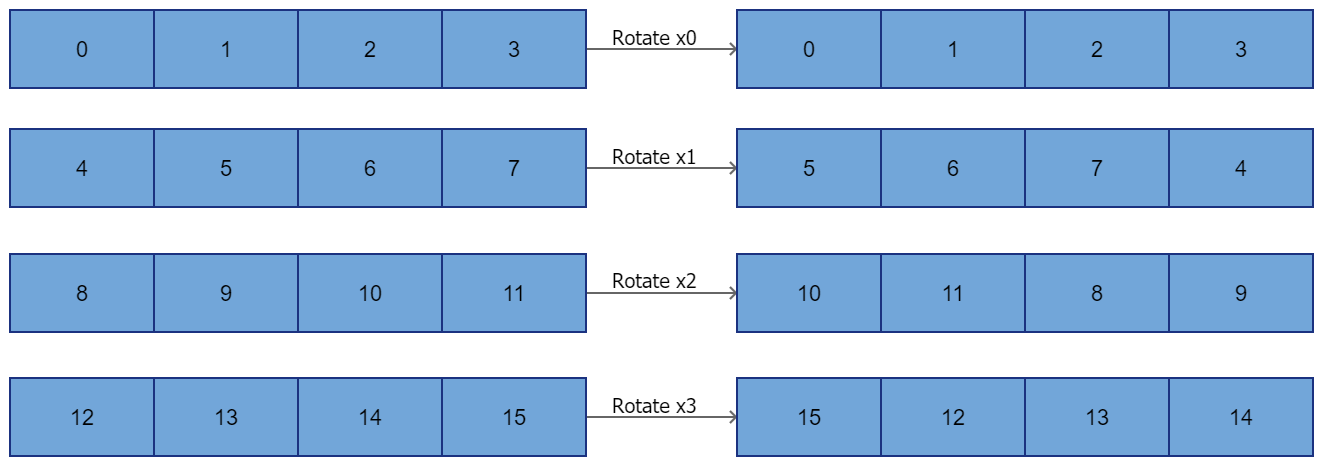
\includegraphics[width=\textwidth]{images/tf3_schema_shiftrow.png}
    \caption{Testfall 3: Schema der ShiftRow-Verschlüsselung}
    \label{fig:tf3-schema}
\end{figure}

\begin{figure}[H]
    \noindent\textbf{Gegeneingabe Entschlüsselung:}\par\vspace{2mm}
    \centering
    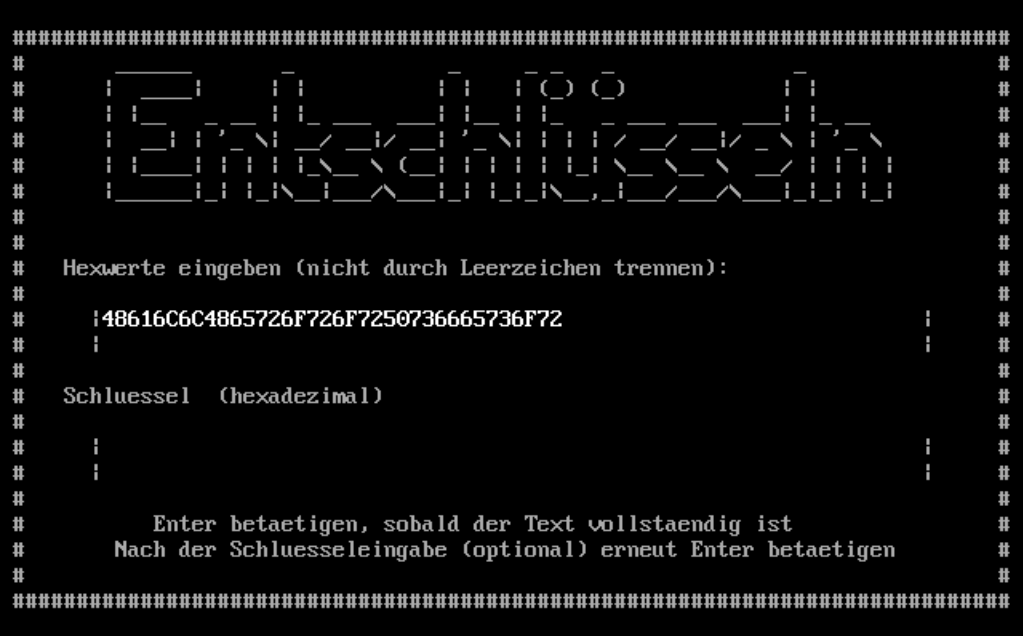
\includegraphics[width=0.72\textwidth]{images/tf3_ent_eingabe.png}
    \caption{Testfall 3: Eingabe des Chiffretextes zum Entschlüsseln}
    \label{fig:tf3-ent-ein}
\end{figure}

\begin{figure}[H]
    \centering
    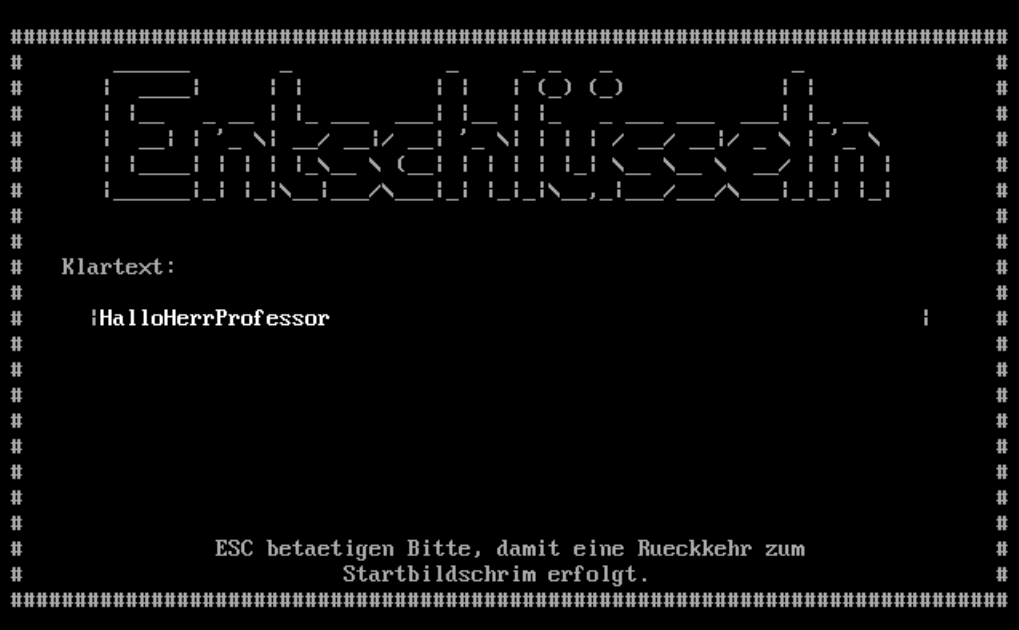
\includegraphics[width=0.72\textwidth]{images/tf3_ent_ergebnis.png}
    \caption{Testfall 3: Ergebnis der Entschlüsselung (ShiftRow invers)}
    \label{fig:tf3-ent-erg}
\end{figure}

%------------------------------------------------------------------------------
\Needspace{14\baselineskip}
\subsection{Testfall 4 -- ShiftColumn}\label{sec:tf4}
\textbf{Stand 2.0.0:} \asm{MalZweiPROC}, auf die \asm{ShiftColumn} aufbaut, wurde korrigiert (Abschnitt~\ref{sec:vers-shiftcolumn}). Die Prüfung gegen die Referenzvektoren steht in Abschnitt~\ref{sec:tests-modell} (M4, M6, M7). Wie damals wird \asm{ShiftColumn} nur in einem Einzeltest, nicht im aktiven Ablauf geprüft.

\begin{figure}[H]
    \centering
    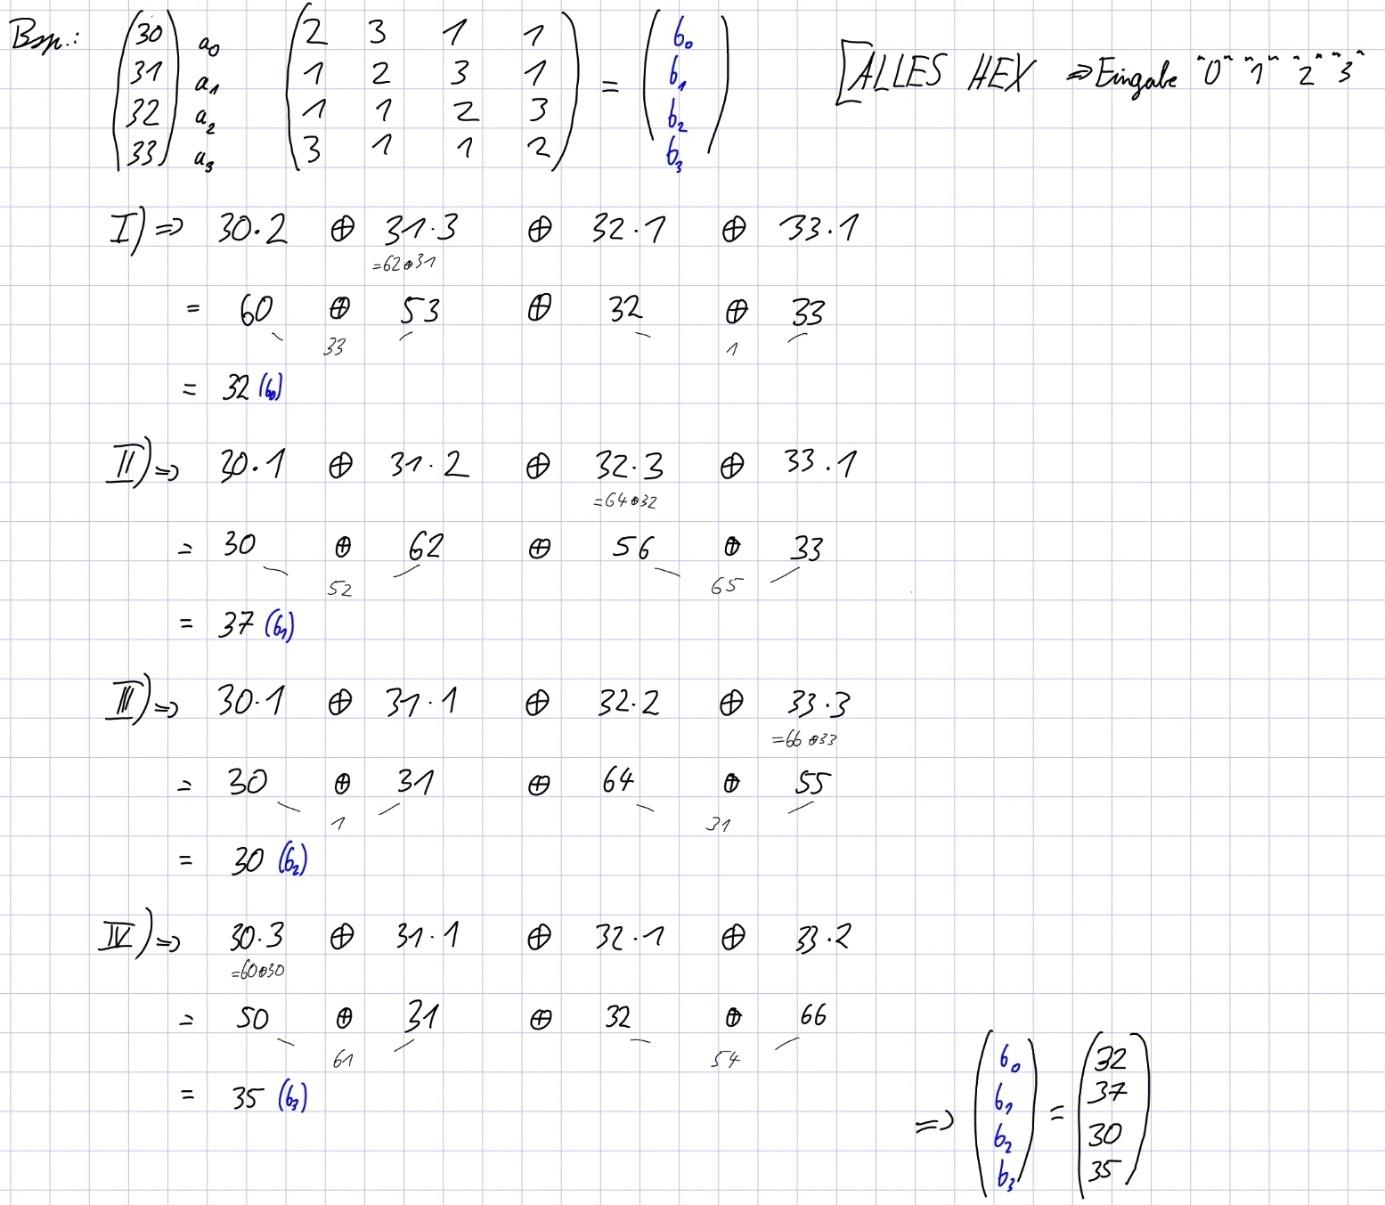
\includegraphics[width=0.95\textwidth]{images/tf4_handrechnung.png}
    \caption{Testfall 4: Handrechnung zur ShiftColumn}
    \label{fig:tf4-hand}
\end{figure}

\begin{figure}[H]
    \noindent\textbf{Screenshot:}\par\vspace{2mm}
    \centering
    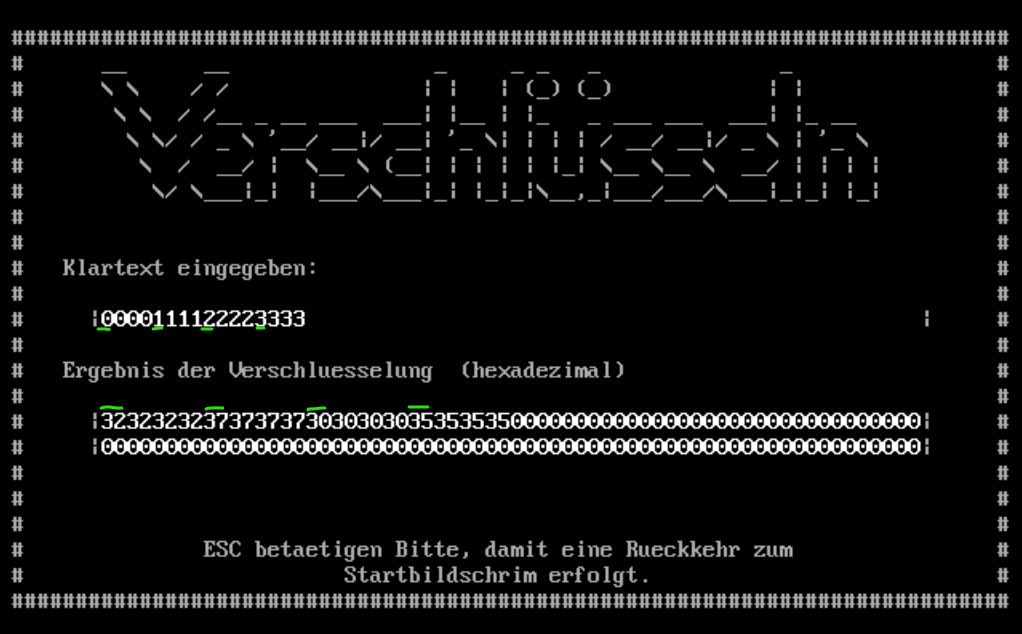
\includegraphics[width=0.72\textwidth]{images/tf4_screenshot.png}
    \caption{Testfall 4: Screenshot des Programmergebnisses}
    \label{fig:tf4-shot}
\end{figure}

%------------------------------------------------------------------------------
\Needspace{14\baselineskip}
\subsection{Testfall 5 -- ShiftColumn Invers}\label{sec:tf5}
Ergebnis in Version~1.x: fehlgeschlagen \iconfehler

\textbf{Stand 2.0.0:} Die PROC wurde neu geschrieben (Kapitel~\ref{sec:asm-dateien}, \asm{ShiftColumn_1}); die Handrechnung unten zeigt noch den damaligen Versuch. Das Ergebnis der neuen Fassung im Modell steht in M5 bis M7 (Abschnitt~\ref{sec:tests-modell}).

\begin{figure}[H]
    \centering
    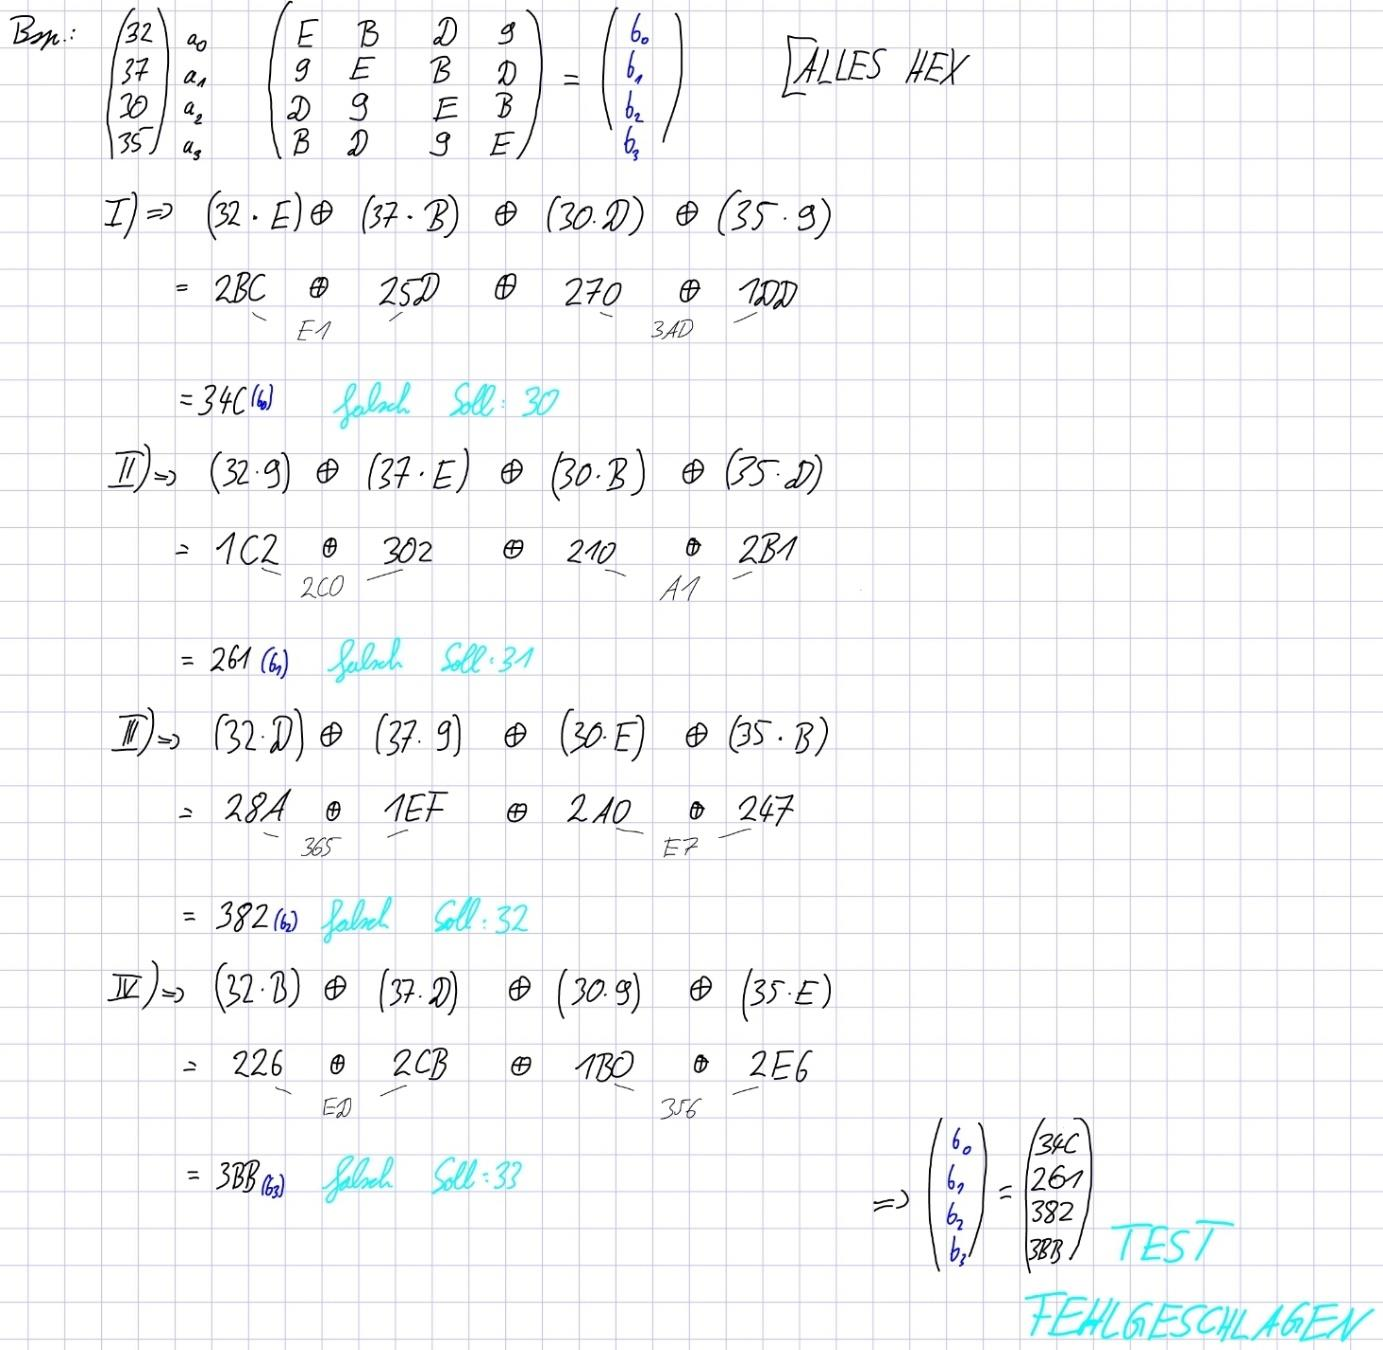
\includegraphics[width=0.95\textwidth]{images/tf5_handrechnung.png}
    \caption{Testfall 5: Handrechnung zur inversen ShiftColumn}
    \label{fig:tf5-hand}
\end{figure}

%------------------------------------------------------------------------------
\Needspace{14\baselineskip}
\subsection{Testfall 6 -- SchluesselAnwenden (PROC)}\label{sec:tf6}
Es wird hier der implementierte Standardschlüssel ohne Expansion verwendet zur Demonstration.

\begin{table}[H]
    \noindent\textbf{Theoretisch:}\par\vspace{2mm}
    \centering
    \small
    \renewcommand{\arraystretch}{1.05}
    \caption{Testfall 6: Anwenden des Standardschlüssels (XOR)}\label{tab:tf6}
    \begin{tabular}{|l|l|l|l|}
        \hline
        \textbf{Buchstabe} & \textbf{HexWert (ASCII)} & \textbf{Schlüsselwert} & \textbf{XOR Ergebnis} \\ \hline
        \sarow{H}{48}{72}{51}{19}
        \sarow{a}{61}{97}{DB}{BA}
        \sarow{l}{6C}{108}{AD}{C1}
        \sarow{l}{6C}{108}{CF}{A3}
        \sarow{o}{6F}{111}{83}{EC}
        \sarow{H}{48}{72}{9F}{D7}
        \sarow{e}{65}{101}{BD}{D8}
        \sarow{r}{72}{114}{27}{55}
        \sarow{r}{72}{114}{B7}{C5}
        \sarow{P}{50}{80}{FF}{AF}
        \sarow{r}{72}{114}{25}{57}
        \sarow{o}{6F}{111}{8A}{E5}
        \sarow{f}{66}{102}{1F}{79}
        \sarow{e}{65}{101}{A6}{C3}
        \sarow{s}{73}{115}{B3}{C0}
        \sarow{s}{73}{115}{91}{E2}
        \sarow{o}{6F}{111}{FB}{94}
        \sarow{r}{72}{114}{9C}{EE}
    \end{tabular}
\end{table}

\begin{figure}[H]
    \noindent\textbf{Screenshot als Beweis:}\par\vspace{2mm}
    \centering
    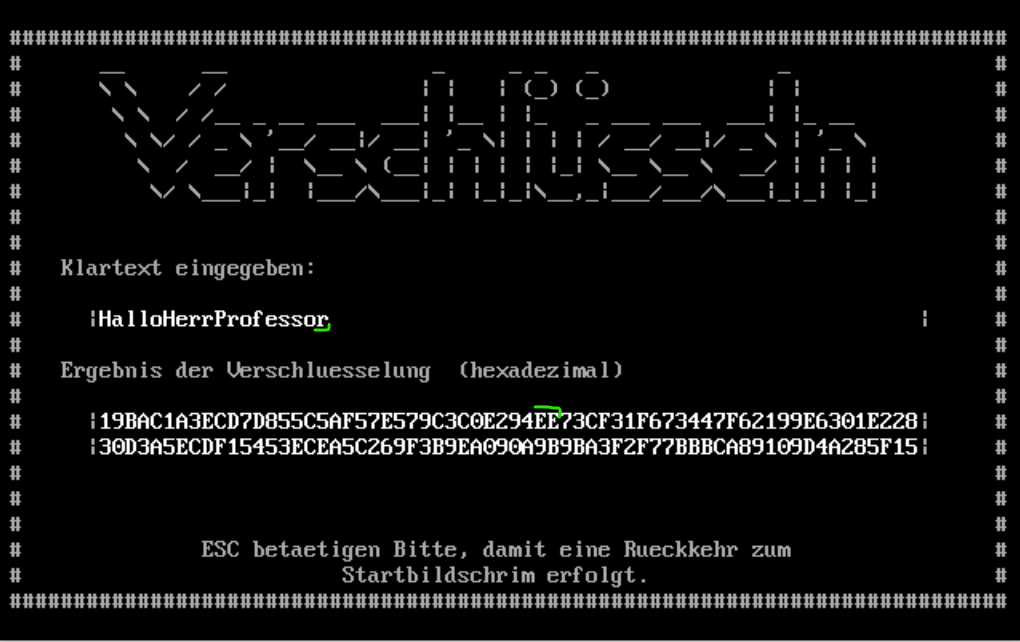
\includegraphics[width=0.72\textwidth]{images/tf6_screenshot.png}
    \caption{Testfall 6: Screenshot als Beweis}
    \label{fig:tf6-shot}
\end{figure}

%------------------------------------------------------------------------------
\Needspace{14\baselineskip}
\subsection{Modellprüfung der Version \versionProjekt}\label{sec:tests-modell}
Zu Version~\versionProjekt\ gehört das Skript \asm{Dokumentation/Modelltest/modelltest.py}. Es bildet die Prozeduren \asm{SchluesselInitialisieren}, \asm{SchluesselAnwenden}, \asm{Schluesselexpansion}, \asm{SBOXSubstitution}, \asm{ShiftRow}, \asm{MalZweiPROC}, \asm{GFMulPROC}, \asm{ShiftColumn} und ihre Gegenstücke Schritt für Schritt (gleiche Register- und Speicherbelegung, gleiche Schleifen) in Python nach und liest die Tabellen direkt aus \asm{SBOX.asm} und \asm{config.asm}. Geprüft wird gegen Referenzen, die nicht aus dem Assemblercode stammen: die AES-S-Box aus ihrer Definition, die Multiplikation in $\mathrm{GF}(2^8)$ per Polynomdivision, Testvektoren aus \cite{fips197} bzw.\ der MixColumns-Literatur und eine Formel für \asm{ShiftRow}.

\begin{table}[!htbp]
    \centering
    \small
    \renewcommand{\arraystretch}{1.1}
    \caption{Modellprüfung -- Ergebnisse von \texttt{modelltest.py}}\label{tab:tests-modell}
    \begin{tabular}{@{}lp{6.2cm}p{5.6cm}@{}}
        \toprule
        \textbf{Nr.} & \textbf{Prüfung} & \textbf{Umfang / Ergebnis} \\
        \midrule
        M1 & S-Box und inverse S-Box gleich der AES-S-Box \cite{fips197} & 256 Einträge je Tabelle \iconok \\
        M2 & \asm{ShiftRow} und \asm{ShiftRow_1}, alle vier Blöcke & 300 Zufallszustände, Block 4 einzeln \iconok \\
        M3 & Schlüsselexpansion & $K_1=$ \asm{65 BE 13 DC}\ldots, $K_2=$ \asm{7A C4 D7 0B}\ldots; Konstante \asm{5F}, \asm{BE}, \asm{7D} \iconok \\
        M4 & \asm{MalZweiPROC} & alle 256 Eingaben \iconok \\
        M5 & \asm{GFMulPROC} & alle 65\,536 Paare \iconok \\
        M6 & \asm{ShiftColumn} und \asm{ShiftColumn_1} gegen Testvektoren & 6 Vektoren (u.\,a. \asm{DB 13 53 45} $\to$ \asm{8E 4D A1 BC}), alle 16 Spalten \iconok \\
        M7 & \asm{ShiftColumn} und Umkehrung, zufällig & 2000 Zustände \iconok \\
        M8 & Verschlüsselung \glqq Hallo\grqq{} & Chiffrat wie in Kapitel~\ref{sec:ablauf-beispiel} \iconok \\
        M9 & Ver- und Entschlüsseln, Standardschlüssel & 500 Zufallstexte \iconok \\
        M10 & Ver- und Entschlüsseln, eigener (Teil-)Schlüssel & 500 Fälle \iconok \\
        M11 & vierter Block wird verarbeitet & \asm{Pos 48}--\asm{63} \iconok \\
        \bottomrule
    \end{tabular}
\end{table}

\textbf{Aussagekraft.} Die Modellprüfung belegt, dass die \emph{Logik} der Assemblerroutinen stimmt. Sie belegt nicht, dass der Quelltext fehlerfrei übersetzt wird, dass die Register im echten Lauf die angenommenen Werte haben (z.\,B.\ \asm{DS}/\asm{ES}) oder dass die Bildschirmausgabe stimmt. Dafür sind die DOS-Box-Tests in Abschnitt~\ref{sec:tests-dosbox} nötig. Beim Schreiben des Skripts fiel auf, dass die Tabelle \asm{s_1_0} einen Eintrag \asm{0D5H} (großes \asm{H}) enthält; Programme, die die Tabelle auswerten, müssen die Groß-/Kleinschreibung des Suffixes beachten (TASM akzeptiert beides).

%------------------------------------------------------------------------------
\Needspace{14\baselineskip}
\subsection{Noch auszuführen: Tests in der DOS-Box (Version \versionProjekt)}\label{sec:tests-dosbox}
Diese Tests sind für Version~\versionProjekt\ noch von Hand durchzuführen (\asm{asmaes.bat}, dann \asm{start.bat}). Die erwarteten Werte stammen aus dem Modell (Teil~B). Die Spalte \glqq Ergebnis\grqq{} ist absichtlich leer.

\begin{table}[!htbp]
    \centering
    \small
    \renewcommand{\arraystretch}{1.15}
    \caption{DOS-Box-Tests für Version \versionProjekt}\label{tab:tests-dosbox}
    \begin{tabular}{@{}lp{3.1cm}p{5.9cm}c@{}}
        \toprule
        \textbf{Nr.} & \textbf{Eingabe} & \textbf{Erwartung} & \textbf{Ergebnis} \\
        \midrule
        D1 & Programm kompilieren und starten & fehlerfrei übersetzt; Hauptbildschirm erscheint & \\
        D2 & Verschlüsseln: \texttt{Hallo}, \asm{Enter}, \asm{Enter} & Chiffrat \asm{E159BDA8 8E0FB958 ...}, vollständig Listing~\ref{lst:beispiel-chiffrat} & \\
        D3 & Entschlüsseln: Chiffrat aus D2, \asm{Enter}, \asm{Enter} & \texttt{Hallo}, dahinter Leerstellen & \\
        D4 & Verschlüsseln: \texttt{Hallo}, eigener Schlüssel \asm{01} $\times 64$ (128 Ziffern \texttt{01}) & beginnt mit \asm{E9B50FF0 A2378E6D}; Entschlüsseln mit demselben Schlüssel liefert \texttt{Hallo} & \\
        D5 & Verschlüsseln: \texttt{Hallo}, Teilschlüssel \texttt{5F} (nur ein Byte) & beginnt mit \asm{3E655D79 1E745EBC} & \\
        D6 & Verschlüsseln: 64 Zeichen, Text siehe unter der Tabelle & beginnt mit \asm{BF3DF6BD FC3592CE}, endet mit \asm{... 97D9733B}; Rückweg liefert den Text & \\
        D7 & Entschlüsseln mit falschem Schlüssel & kein \texttt{Hallo}, nur Zeichensalat & \\
        \bottomrule
    \end{tabular}
\end{table}

Der Text für D6 ist \texttt{ABCDEFGHIJKLMNOPQRSTUVWXYZ} gefolgt von \texttt{abcdefghijklmnopqrstuvwxyz} und \texttt{0123456789+-} (zusammen 64 Zeichen, ohne Leerzeichen).

D6 prüft insbesondere den vierten Block (\asm{Pos 48}--\asm{63}), der bei Version~1.0 nicht verschoben wurde. D4 und D5 prüfen die Schlüsseleingabe, die bis Version~1.0 wirkungslos war. Erst nach Abarbeitung dieser Tabelle ist Version~\versionProjekt\ im eigentlichen Sinn getestet.

